\subsection{Descripci\'on del Escenario}
	\par En este escenario se monitorearon los paquetes ARP de la red Wi-Fi de acceso público de un local de comida rápida en una zona muy concurrida de la ciudad de Buenos Aires, un Starbucks en Av. Callao.

	\par A la hora del análisis, se desconoce la naturaleza de la red, quienes intervienen en la misma y el accionar de los usuarios en ella.
    
    \par Se espera que en general las conexiones de los diversos dispositivos de quienes se encuentran en el local sea de algunos pocos minutos y busque simplemente acceder a internet, por lo cual se espera que la principal conmutación se de entre las IPs de estos dispositivos y el \emph{gateway}.


\subsection{An\'alisis de datos obtenidos}
	\par La captura fue de 45 minutos y se enviaron 947 paquetes, el grafo dirigido de conexiones que se obtuvo fue el siguiente:

 %[-Grafo-]
 
\begin{figure}[H]
		\centering
		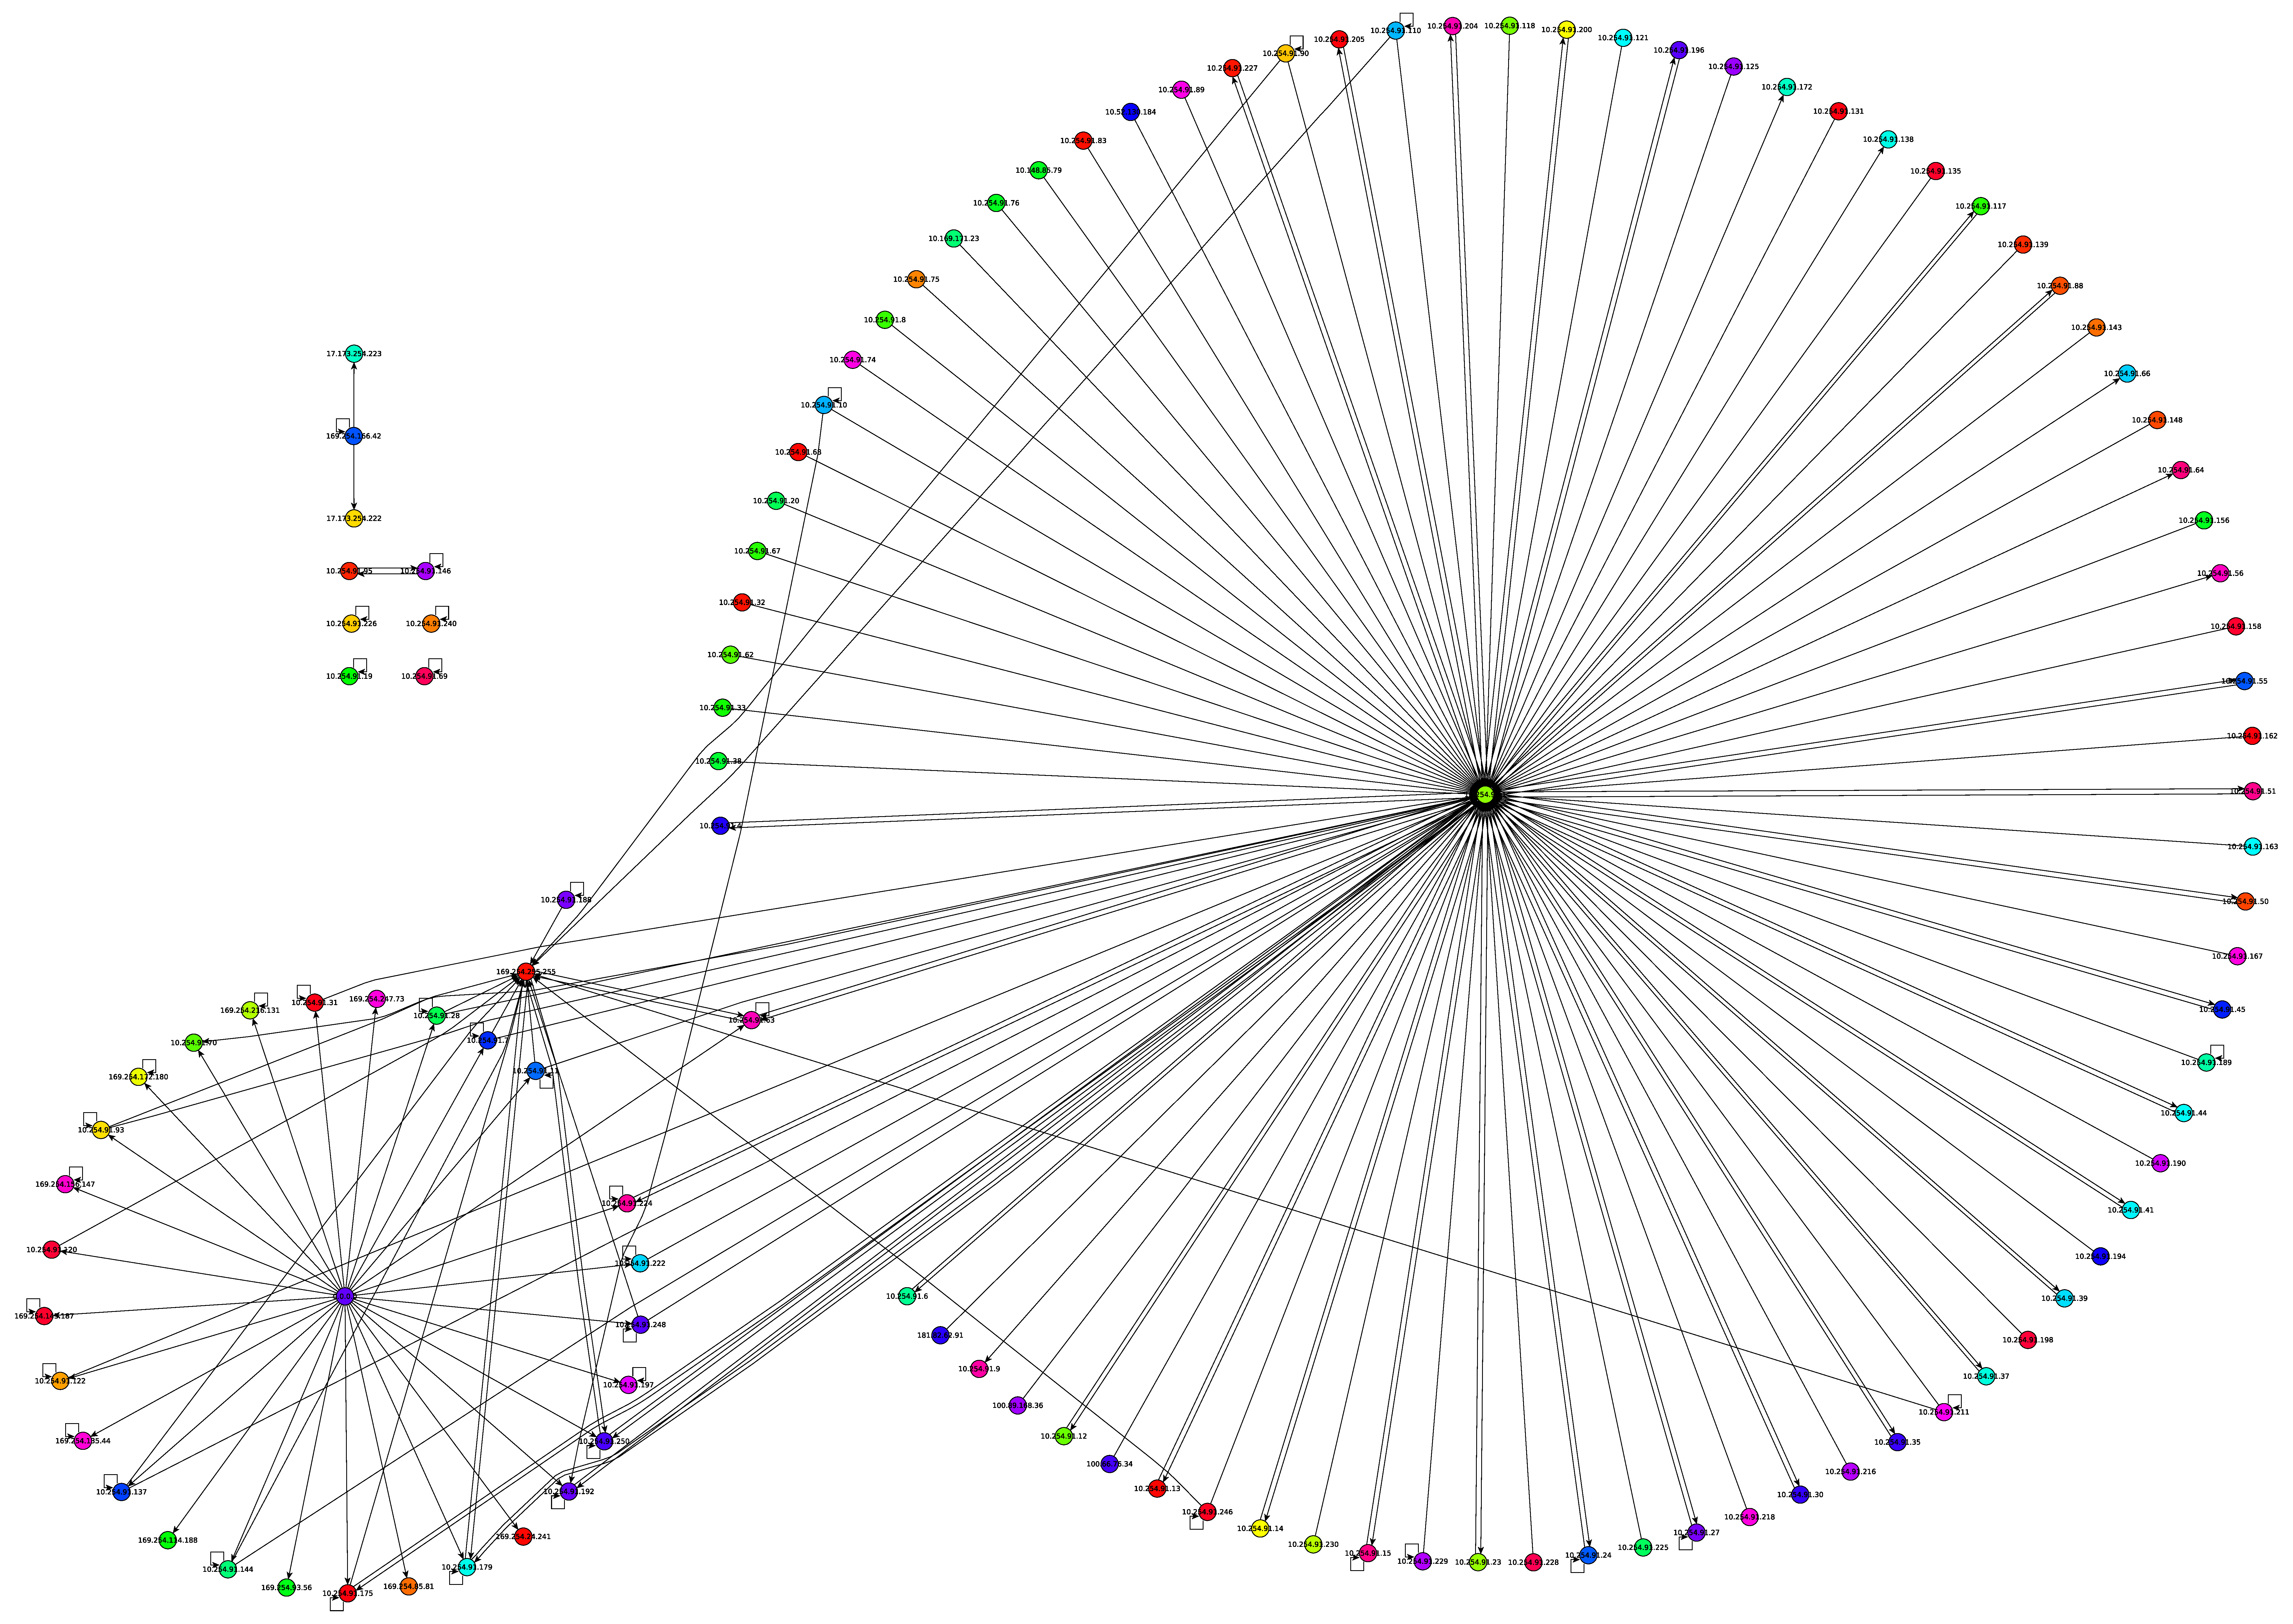
\includegraphics[width=0.5\textwidth]{img/graph/escenario_3/starbucks2.eps}
		\caption{Grafo de la red del Escenario 3}
		\label{fig:grafo_escenario3}
	\end{figure}

		\par Como el grafo es de gran tamaño vamos a considerar subgrafos donde se encuentran nodos interesantes para el análisis.

	\par Hay dos direcciones involucradas en gran parte del tráfico de paquetes, 10.254.91.1 que  recibe y envia hacia una gran cantidad de IPs y 169.254.255.255 que principalmente es destino.

	\par La primera se comporta como el gateaway, interactua con la mayoria de las IPs y es la más activa de toda la red.   Como se ve ampliando la figura 1, la cantidad de direcciones que le envian paqueteses increiblemente grande.

%[-Zoom a IP 10.254.91.1-]

\begin{figure}[H]
		\centering
		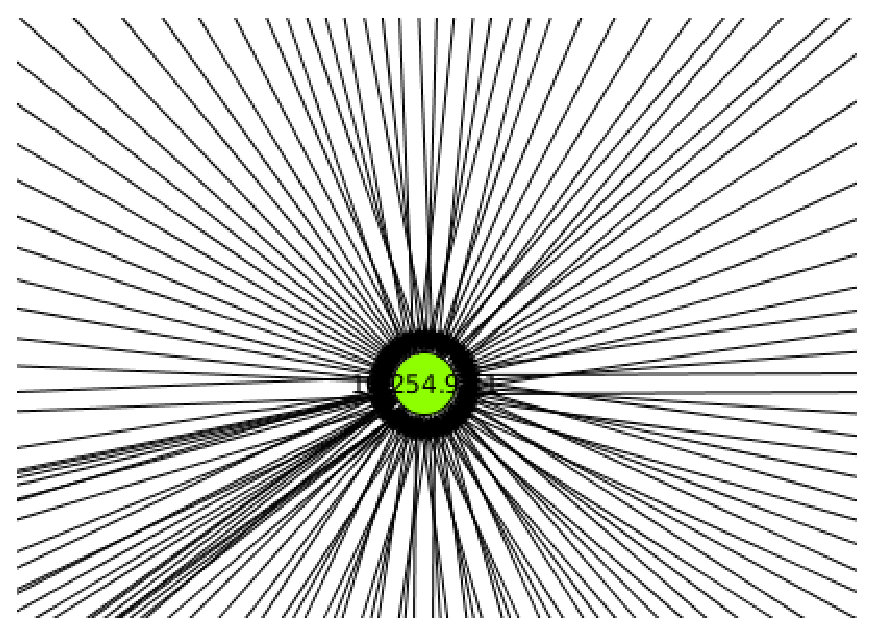
\includegraphics[width=0.5\textwidth]{img/graph/escenario_3/10254.eps}
		\caption{Ampliación en la cercan\'ia a 10.254.91.1}
		\label{fig:gateway_escenario3}
\end{figure}
	\par Tras investigar un poco al respecto, encontramos que la segunda IP mencionada es una dirección reservada  a la que los dispositivos envian paquetes ARP al no encontrar el servidor DHCP ya sea por recien conectarse o perder la ruta hacia el , el dispositivo se asigna una direccion para acceder y comunicarse a la red que usará hasta que se le asigne una IP mediante DHCP. \footnote{http://www.ietf.org/rfc/rfc3927.txt}
	\par Si nos quedamos solamente con aquellos hosts que interactúan con 169.254.255.255 se obtiene el siguiente grafo:   

%[-Vecindad de la IP 169.254.255.255-]
\begin{figure}[H]
		\centering
		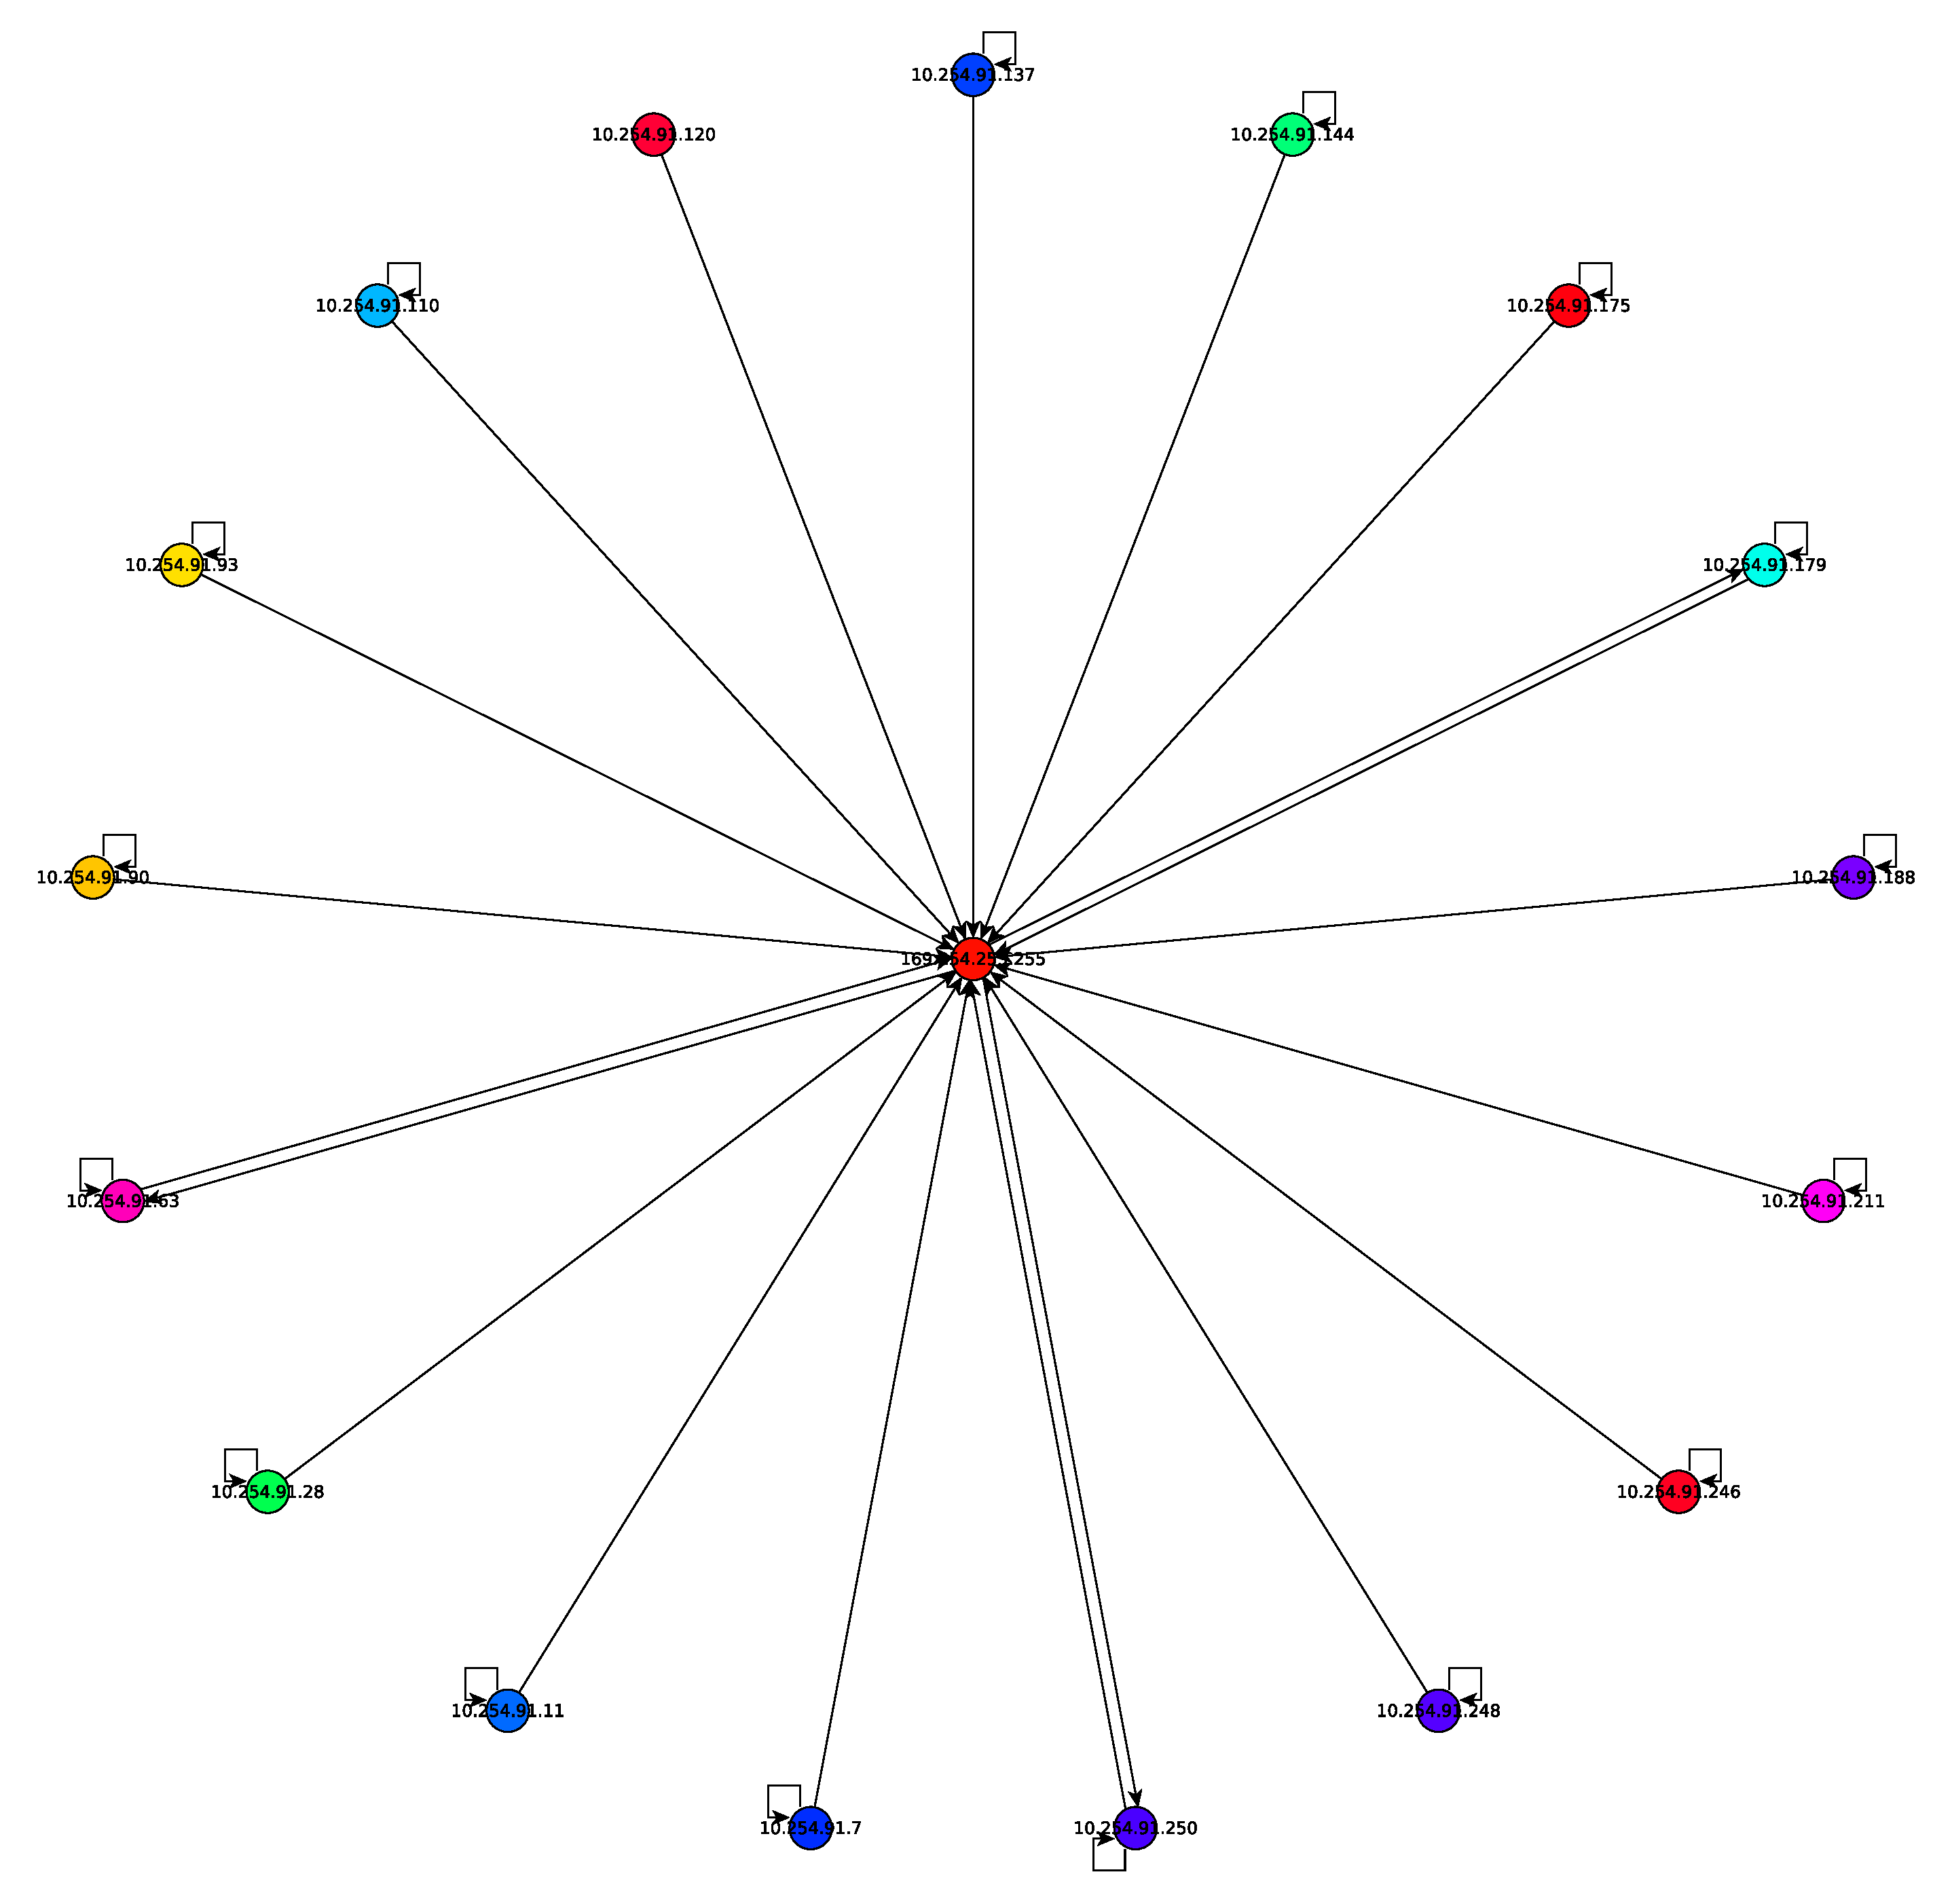
\includegraphics[width=0.5\textwidth]{img/graph/escenario_3/169254_aislado.eps}
		\caption{Vecindad de la IP 169.254.255.255}
		\label{fig:v1_escenario3}
\end{figure}
	\par Tambien se destaca que hay varios paquetes con origen 0.0.0.0, esto se da porque  al conectarse a la red ciertos dispositivos  envian broadcast para ser detectados por el servidor DHCP y que se les asigne una IP, luego terminan recibiendo paquete ARP con la IP asignada.
    
    \par De la misma forma que hicimos antes, se puede generar el grafo de la vecindad a 0.0.0.0 y resulta similar al presentado anteriormente.
    
%[-Vecindad de la IP 0.0.0.0-]
\begin{figure}[H]
		\centering
		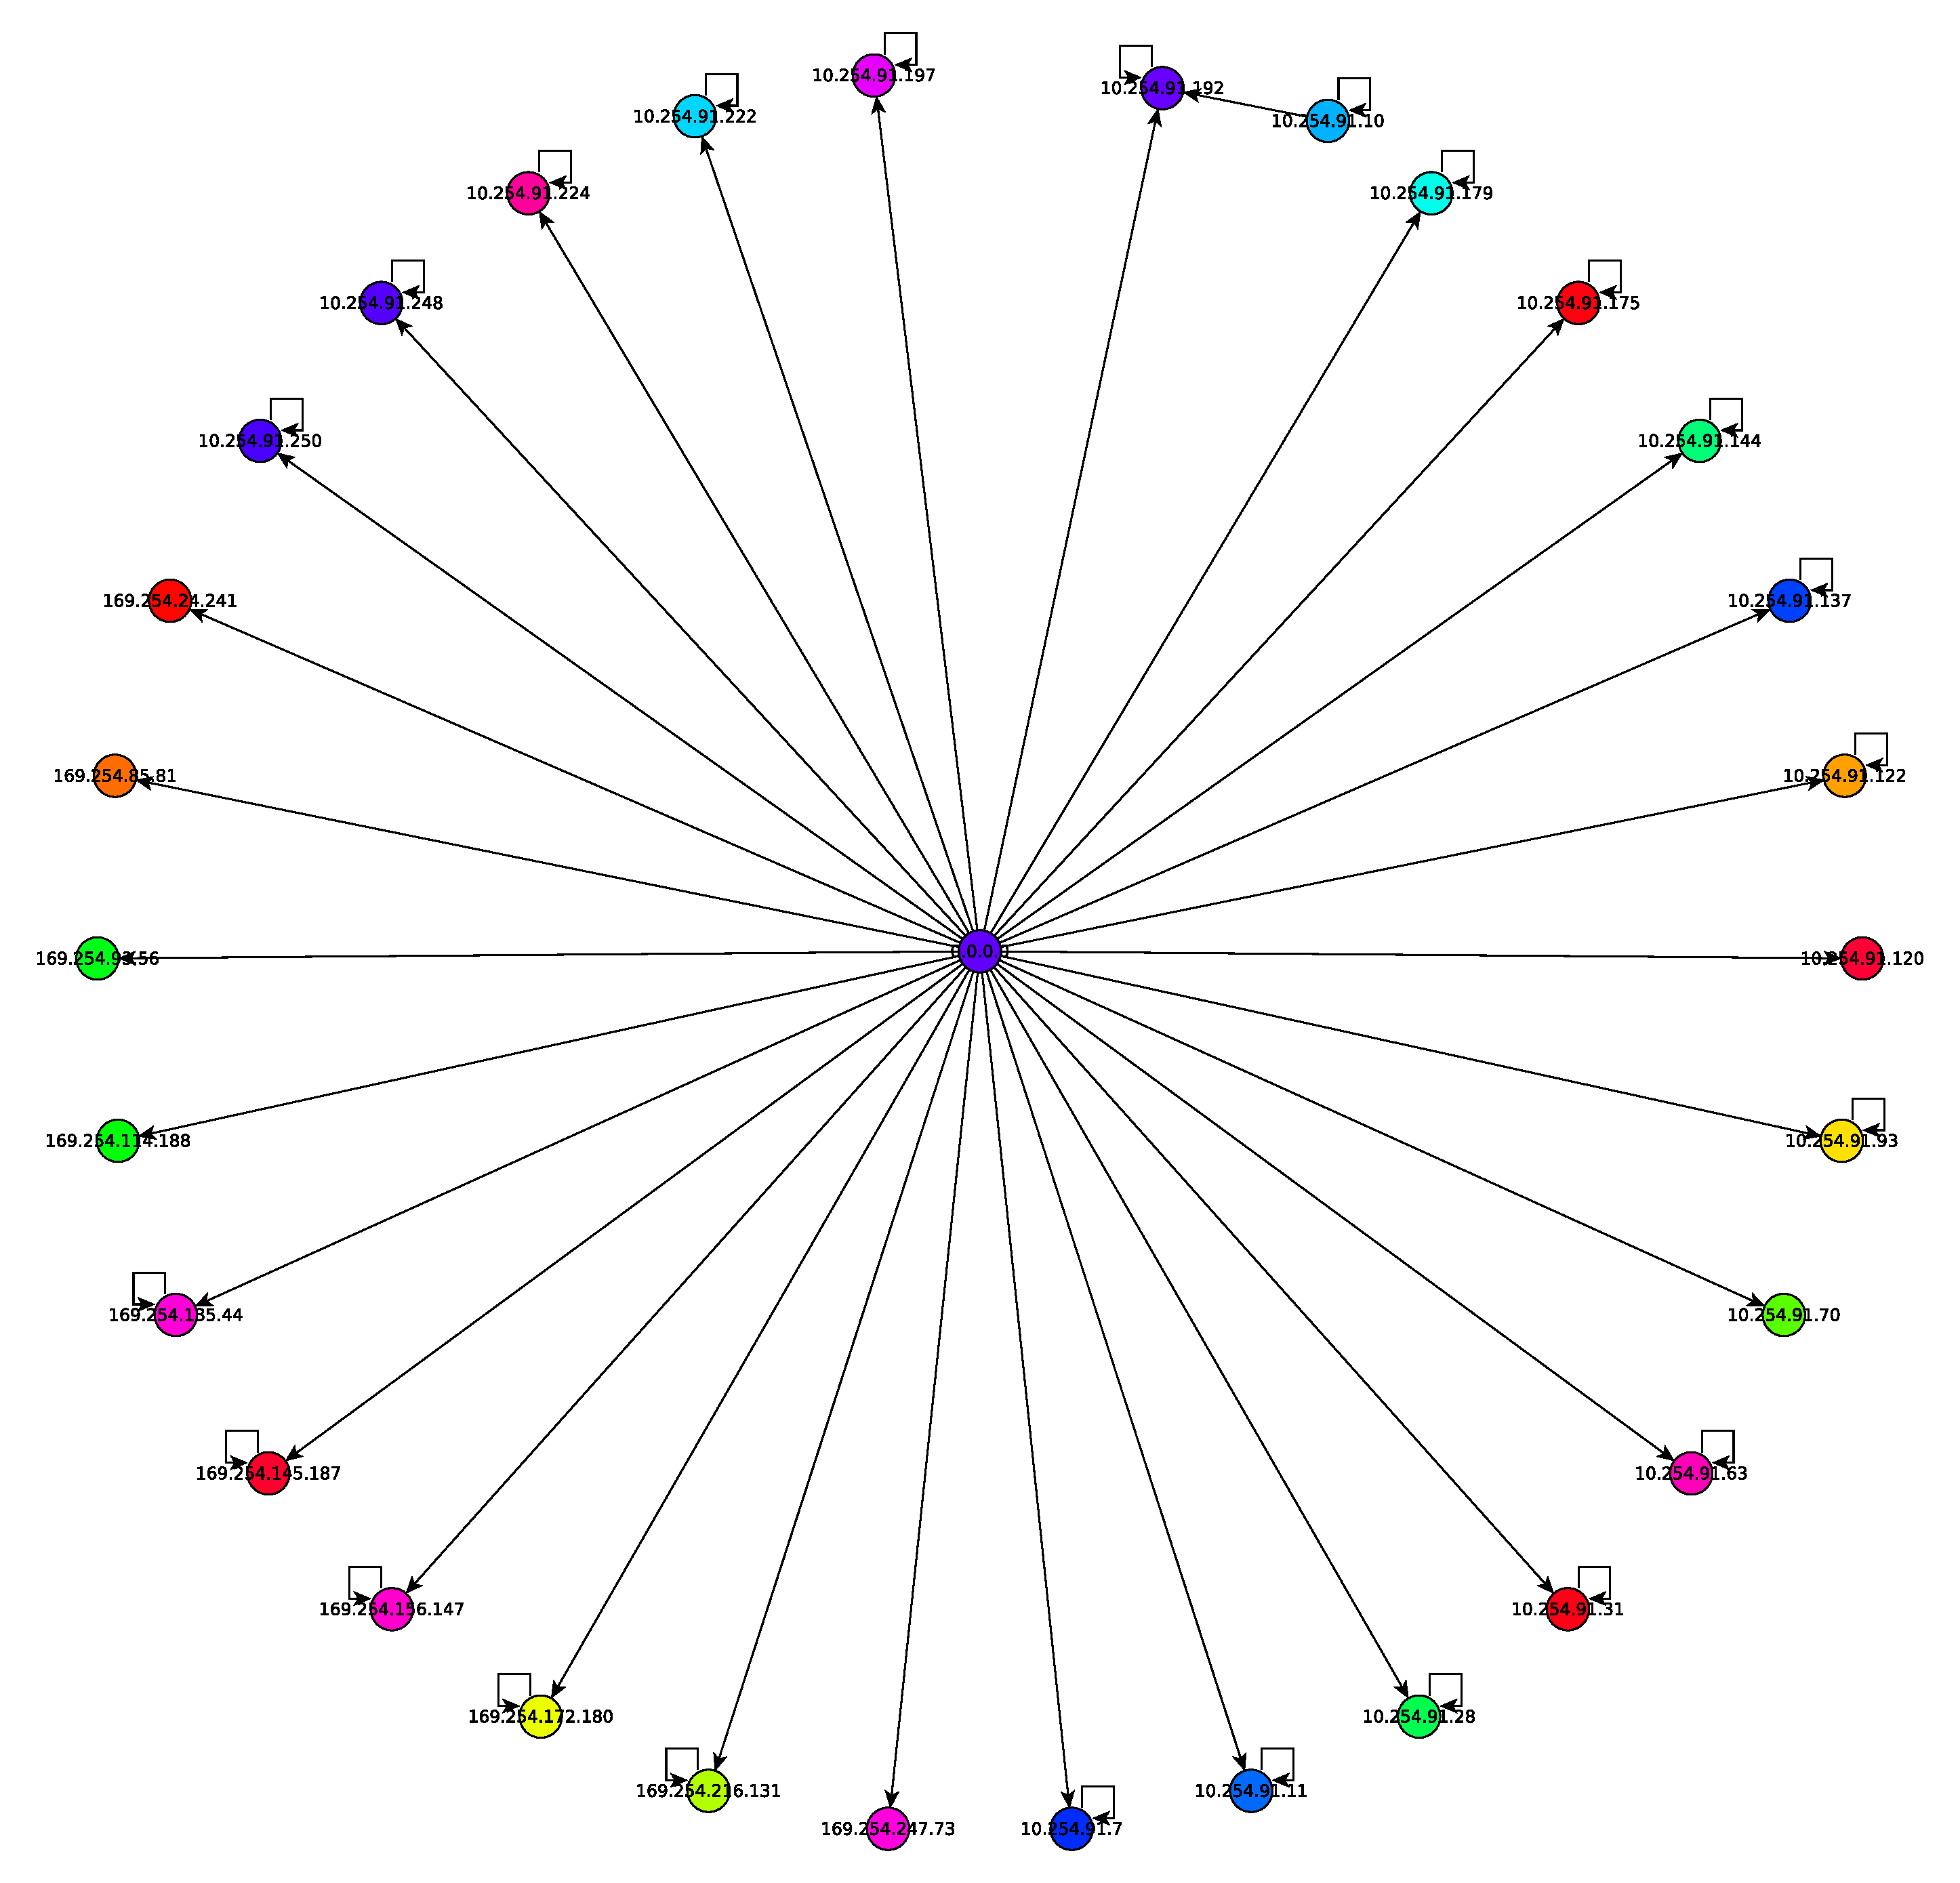
\includegraphics[width=0.5\textwidth]{img/graph/escenario_3/0000_aislado.eps}
		\caption{Vecindad de la IP 0.0.0.0}
		\label{fig:0_escenario3}
\end{figure}

	\par Al solo restringirnos a estos nodos, podemos ver que varios hosts se encontraban en esta situación.
\vspace{6 mm}

	\par El resto de las direcciones se encuentran en el rango 10.254.0.0/16, lo cual es completamente razonable y 169.254.0.0/16 que es un caso más interesante, estas direcciones son conocidas como \emph{Link-local addresses}, son direcciones reservadas asignadas en Windows cuando no se puede establecer contacto con el servidor DHCP y se genera su propia IP mediante el direccionamiento conocido como APIPA. \footnote{http://wiki.wireshark.org/APIPA}

	\par El sistema operativo intentará constantemente conectarse con DHCP y recibir una IP válida, mientras tanto los hosts con estas direcciones pueden comunicarse entre sí dentro de la red, pero no con ninguno externo a la red local.
\vspace{6 mm}
	\par Algunas otras caracteristicas del grafo son:

\begin{itemize}

\item Nodos Aislados:

\par En el grafo se presentan nodos que podemos definir como aislados dado que no se comunicaron con el gateway y no son conexos  al resto del grafo.
    
\par Estos dispositivos se comunican entre sí, con si mismos, o con nadie como es el caso de 17.173.254.223 que no envia paquetes.

\par  Como es minimamente necesario que envien un paquete a 10.254.91.1 luego de ingresar a la red, nos hace suponer que el host se encontraba conectado a la red antes de hacer el análisis y de esta forma obtuvieron su direccion.  
\end{itemize}

%[-Subgrafo con nodos aislados-]
\begin{figure}[H]
		\centering
		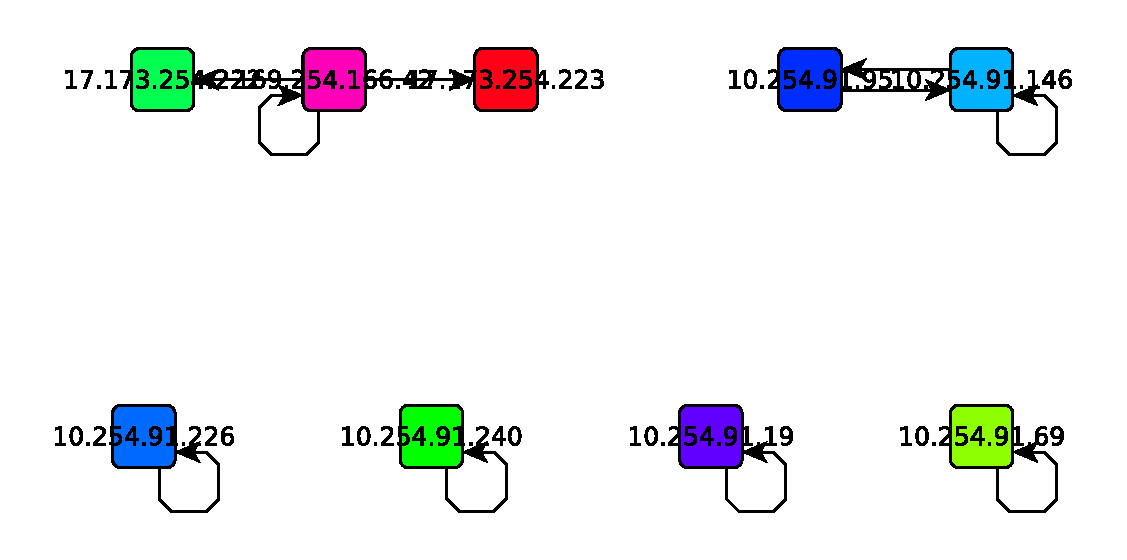
\includegraphics[width=0.5\textwidth]{img/graph/escenario_3/nodos_aislados.eps}
		\caption{Nodos considerados como aislados}
		\label{fig:aislados_escenario3}
\end{figure}


\begin{itemize}
\item Nodos Reflexivos:
\par Podemos notar que algunos nodos envían paquetes a si mismos, algunos motivos por los que puede suceder esto es para actualizar la tabla ARP, para buscar duplicados de la direccion IP o cambios de la direccion MAC. Este envío de paquetes se conoce como Gratuitous ARP.  \footnote{http://wiki.wireshark.org/Gratuitous\_ARP}
\end{itemize}

\subsubsection{Informaci\'on y Entrop\'ia}
		        
	\par En cuanto al análisis de la información de cada simbolo de ambas fuentes, primero calculamos la probabilidad muestral de ambas fuentes.
	\par Las siguientes tablas muestran las 5 IPs con mayor probabilidad muestral obtenidas, tanto para la fuente $S_{src}$ como para $S_{dst}$, decidimos mostrar solo cinco en el orden decreciente ya que a partir de las siguientes la diferencia es menor a 0.005 y se hace imposible apreciarlo en los graficos.

\newpage

\begin{figure}[!ht]
    \centering
    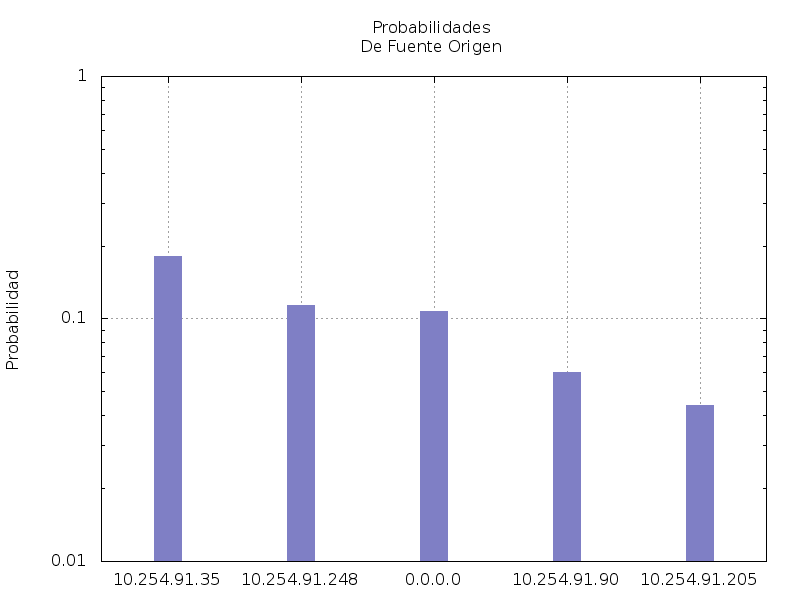
\includegraphics[width=0.5\textwidth]{img/graph/escenario_3/proba_src.png}
\end{figure}


\begin{figure}[!ht]
    \centering
    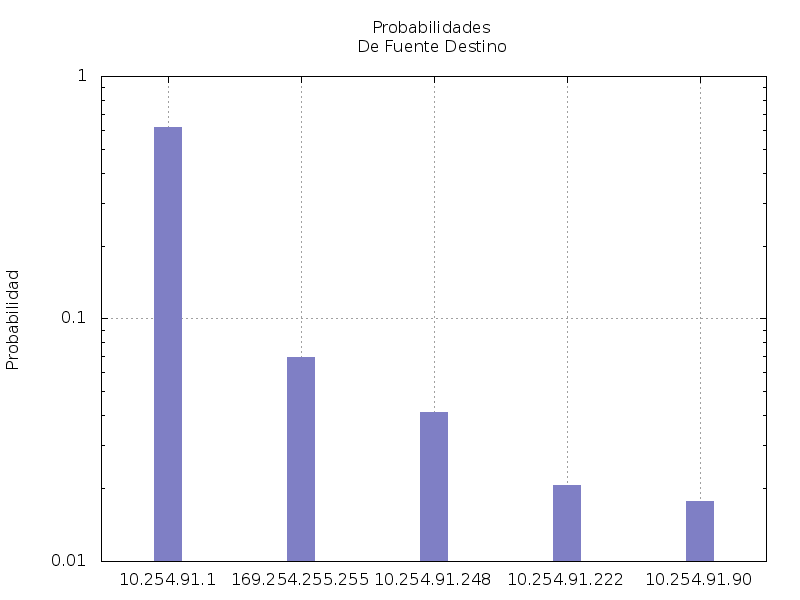
\includegraphics[width=0.5\textwidth]{img/graph/escenario_3/proba_dst.png}
\end{figure}


	\par Para los paquetes de destino, los resultados se corresponden con lo visto al hacer el grafo tanto en los valores de probabilidad como en la proporcionalidad con las demas direcciones, 10.254.91.1 tiene una probabilidad tan alta, que hace necesario mostrar el grafico en escala logaritmica para poder apreciar los valores del resto de las probabilidades. Algo similar a lo que sucede con el grafo, donde la mayoría de los paquetes eran enviados a dicha dirección.
	\vspace{6 mm}

	\par En el caso de la fuente destino, no encontramos ningun comportamiento visto anteriormente, los valores nos muestran que todas las direcciones se acercaron a la media general de envíos de paquetes, inclusive la direccion 0.0.0.0, que al ver el grafo imaginamos que era quien más envios habia realizado. 


	\par A partir de estos valores podemos ver el nivel de información que nos da cada una de estas IPs.

	\par Como ya sabemos la información de cada simbolo $p_{i}$ se obtiene al calcular:

\begin{equation}
	\log_2 (\frac{1}{ p_{i} })
\end{equation}

	\par Al ser una función decreciente, aquellas direcciones del grafico anterior con mayor probabilidad son las de menor información:

\begin{figure}[!ht]
    \centering
    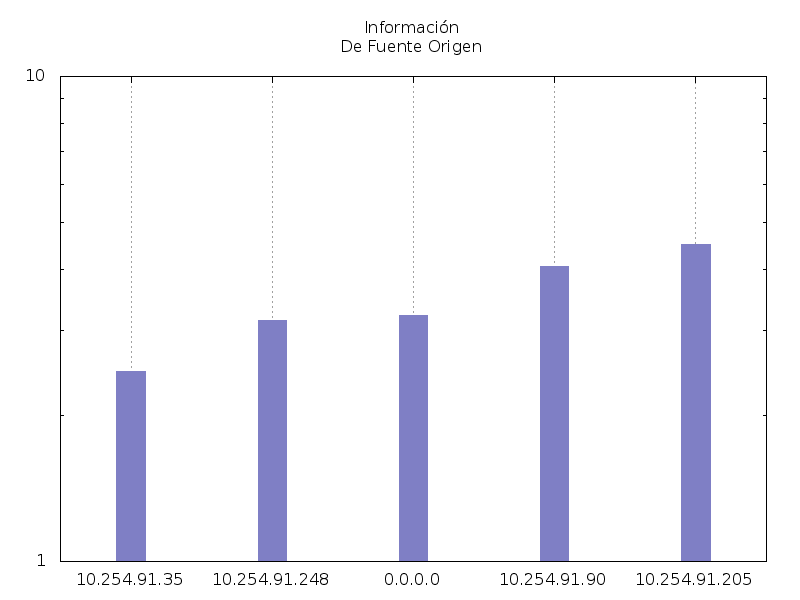
\includegraphics[width=0.5\textwidth]{img/graph/escenario_3/info_src.png}
\end{figure}


\begin{figure}[!ht]
    \centering
    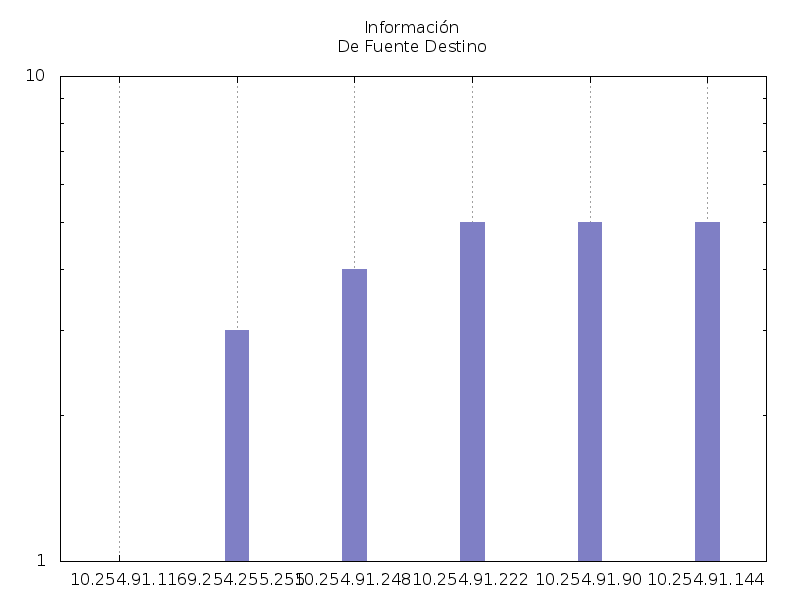
\includegraphics[width=0.5\textwidth]{img/graph/escenario_3/info_dst.png}
\end{figure}

	\par Tanto para este caso como sucedía con las probabilidades, estos son los valores mas significativos y podemos ver que como el router da una cantidad tan baja de informacion la entropia de $S_{src}$ sera mucho menor a la de $S_{dst}$.

	\par Efectivamente eso se da al calcular la media de la información:
    
\vspace{6 mm}

\begin{center}
\begin{tabular}{|c|c|}
\hline
Fuente $S$ & Entropía $H(S)$\\
\hline
$S_{src}$ & 4.96757\\
$S_{dst}$ & 2.8455\\
\hline
\end{tabular}
\end{center}

\subsection{Conclusiones Preliminares}

\par En base a lo visto podemos decir que mediante lo obtenido en la captura pudimos determinar los nodos distinguidos de esta red, al menos para este caso donde solo parece haber un router el símbolo de las fuentes con menor información coincidió con su dirección.
